\section{Auswertung}

Für die Berechnung
der Wellenlängen und Energien werden die Formeln \eqref{eqn:Wellenlänge}
und \eqref{eqn:Winkel} verwendet. Dabei werden sie in
folgende Form umgestellt, wobei n aus Formeln \eqref{eqn:Lambda} das betrachtete
Beugungsmaximum beschreibt (welches im Folgenden immer das 1. ist).

\begin{align}
  \label{eqn:Lambda}
  \lambda\ua{min} &= 2 \cdot d \cdot \sin{\theta} \cdot \frac{1}{n} \\
  \label{eqn:Energie}
  E\ua{max} &= \frac{h \cdot c}{\lambda} \\
\end{align}

\subsection{Überprüfung der Bragg-Bedingung}

Bei der Überprüfung der Bragg-Bedingung werden in dem verwendeten Messprogramm
folgende Einstellungen für den Kristallwinkel $\vartheta$, das Zählrohrwinkelintervall
$\alpha\ua{GM}$, den Winkelzuwachs $\increment\alpha$ sowie die Integrationszeit
$\increment t$ gewählt:

\begin{align*}
  \vartheta        &= 14 \,° \\
  \increment\alpha &= 0.1\, ° \\
  \increment t     &= \SI{10}{s} \\
  \alpha\ua{GM}    &\in [26\, °, 30\, °] .
\end{align*}

Mithilfe von Python und der Daten aus Abbildung \ref{fig:MessungA} sowie Tabelle
\ref{tab:Messung3.1} wird dann das Maximum der
Impulsrate bestimmt. Der Winkel wird dann zuerst in die minimale Wellenlänge (Formel
\eqref{eqn:Lambda}) sowie
anschließend in die maximale Energie (Formel \eqref{eqn:Energie}) umgerechnet,
so dass sich folgende Werte ergeben:

\begin{align*}
  \vartheta\ua{3.1,max} &= 28,6\, ° \\
  \lambda\ua{3.1,min} &= \SI{1.93e-10}{m} \\
  E\ua{3.1, max} &= \SI{6.43}{eV} .
\end{align*}

\begin{figure}
  \centering
  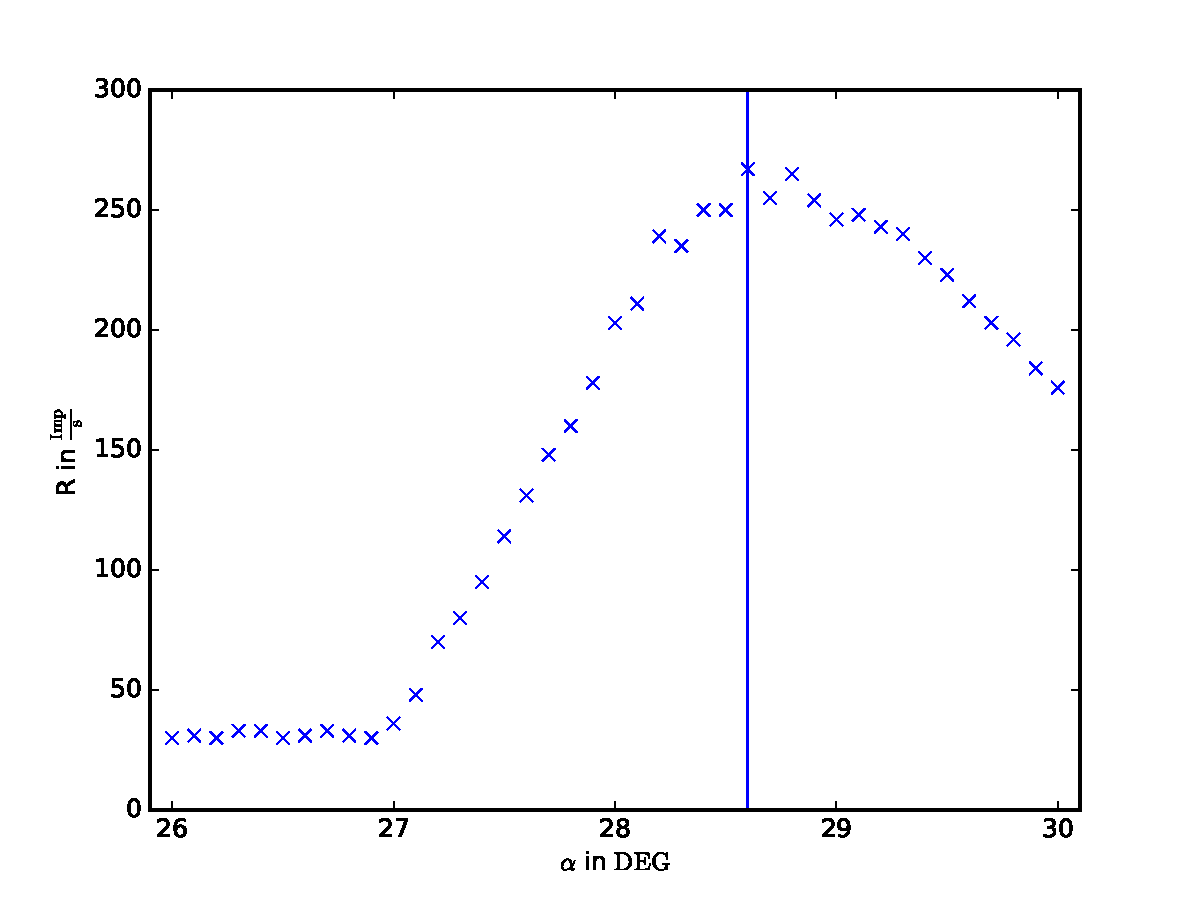
\includegraphics[width = 0.8\textwidth]{Python/MessungA.pdf}
  \caption{Gemessene Impulsrate bei Messung 3.1 .}
  \label{fig:MessungA}
\end{figure}

Im Vergleich mit dem Erwartungswert von $\vartheta$ = 28 ° ergibt sich für den
gemessenen Wert eine
Abweichung von $\increment\vartheta$ = 0.6 ° sowie prozentual eine Abweichung
von $\increment\vartheta$ = 2.1 $\%$.

\begin{table}
  \centering
  \caption{Gemessene Impulsraten N bei Messung 3.1 .}
  \label{tab:Messung3.1}
  \begin{tabular}{c c | c c | c c}
    \toprule
    2$\vartheta$ in deg & N in $\frac{\su{Imp}}{\su{s}}$ & 2$\vartheta$ in deg &
    N in $\frac{\su{Imp}}{\su{s}}$ & 2$\vartheta$ in deg & N in $\frac{\su{Imp}}{\su{s}}$ \\
    \midrule
    26.0 & 30.0 & 27.4 & 95.0  & 28.8 & 265.0 \\
    26.1 & 31.0 & 27.5 & 114.0 & 28.9 & 254.0 \\
    26.2 & 30.0 & 27.6 & 131.0 & 29.0 & 246.0 \\
    26.3 & 33.0 & 27.7 & 148.0 & 29.1 & 248.0 \\
    26.4 & 33.0 & 27.8 & 160.0 & 29.2 & 243.0 \\
    26.5 & 30.0 & 27.9 & 178.0 & 29.3 & 240.0 \\
    26.6 & 31.0 & 28.0 & 203.0 & 29.4 & 230.0 \\
    26.7 & 33.0 & 28.1 & 211.0 & 29.5 & 223.0 \\
    26.8 & 31.0 & 28.2 & 239.0 & 29.6 & 212.0 \\
    26.9 & 30.0 & 28.3 & 235.0 & 29.7 & 203.0 \\
    27.0 & 36.0 & 28.4 & 250.0 & 29.8 & 196.0 \\
    27.1 & 48.0 & 28.5 & 250.0 & 29.9 & 184.0 \\
    27.2 & 70.0 & 28.6 & 267.0 & 30.0 & 176.0 \\
    27.3 & 80.0 & 28.7 & 255.0 &      &       \\
    \bottomrule
  \end{tabular}
\end{table}


\subsection{Das Emissionsspektrum einer Cu-Röntgenröhre}

Für die Untersuchung des Emissionsspektrums einer Cu-Röntgenröhre wurden in dem
2:1 Koppelmodus die folgenden Einstellungen gewählt:

\begin{align*}
  \vartheta        &\in [4 \,°, 26\, °]  \\
  \increment\vartheta &= 0.2 \,° \\
  \increment t     &= \SI{5}{s} .
\end{align*}

Die erhaltenen Daten sind in Abbildung \ref{fig:MessungB} dargestellt. Zur Bestimmung der
$K\ua{\alpha}$- und $K\ua{\beta}$-Linie wird zuerst der Untergrund aus den Daten
herausgerechnet. Dafür wird an die Werte in Tabelle \ref{tab:Untergrund} ein Polynom 3.Ordnung
gefittet, für das sich die folgenden Parameter ergeben:

\begin{align*}
  U(x) &= A\cdot x^3 + B\cdot x^2 + C\cdot x + D \\
  A &=  (0.27 \pm 0.02) \, \si{\frac{Imp}{s\cdot \alpha^3}} \\
  B &= (-12.2 \pm -0.7) \, \si{\frac{Imp}{s\cdot \alpha^2}} \\
  C &= (170 \pm 9) \, \si{\frac{Imp}{s\cdot \alpha}} \\
  D &= (-525 \pm 31) \, \si{\frac{Imp}{s}} .
\end{align*}

Des weiteren wird an die Daten aus Tabelle \ref{tab:Gauß1} eine Gauß-Funktion
der Form \eqref{eqn:GaußFit} gefittet. Dabei werden mithilfe der
Werte des Untergrunds noch die Daten der Tabelle vor dem Fitten angepasst.

\begin{equation}
  G(x) = A\ua{K\ua{\alpha}} \cdot \exp{ \frac{-(\vartheta-\vartheta\ua{K\ua{\alpha}})^2}{2\cdot s\ua{K\ua{\alpha}}^2}}
      + A\ua{K\ua{\beta}} \cdot \exp{ \frac{-(\vartheta-\vartheta\ua{K\ua{\beta}})^2}{2\cdot s\ua{K\ua{\beta}}^2}}
  \label{eqn:GaußFit}
\end{equation}

$\vartheta_K$ und $s$ geben dabei die Lage der jeweiligen Linie sowie die
Standardabweichung an. Damit ergeben sich für die $K\ua{\alpha}$-Linie die folgenden
Parameter:

\begin{align*}
  A\ua{K\ua{\alpha}} &= (4.7 \pm 0.2) \cdot 10^3 \, \si{\frac{Imp}{s}} \\
  \vartheta\ua{K\ua{\alpha}} &= \vartheta_0 =  (22.568 \pm 0.008) \,° \\
  \lambda\ua{K\ua{\alpha}} &= (1.5459 \pm 0.0005) \cdot 10^{-10} \, \si{m} \\
  E\ua{K\ua{\alpha}} &= (8020 \pm 3) \, \si{eV} \\
  s\ua{K\ua{\alpha}} &= (0.39 \pm 0.02) \,° .
\end{align*}

Analog ergeben sich für die $K\ua{\beta}$-Linie die folgenden Werte :

\begin{align*}
  A\ua{K\ua{\beta}} &= (1.6 \pm 0.3) \cdot 10^3 \, \si{\frac{Imp}{s}} \\
  \vartheta\ua{K\ua{\beta}} &= \vartheta_0 =  (20.29 \pm 0.02)\, ° \\
  \lambda\ua{K\ua{\beta}} &= (1.397 \pm 0.001) \cdot 10^{-10} \, \si{m} \\
  E\ua{K\ua{\beta}} &= (8877 \pm 8) \, \si{eV} \\
  s\ua{K\ua{\beta}} &= (0.28 \pm 0.05) \,° .
\end{align*}

\begin{equation}
  E\ua{K\ua{\alpha}} = R\ua{\infty} (z - \sigma\ua{1})^2 - R\ua{\infty} (z - \sigma\ua{2})^2 \cdot \frac{1}{2}.
  \label{eqn:KundLKante}
\end{equation}

Mithilfe der Formeln \ref{eqn:KundLKante} können dann die Abschirmkonstanten der K-Kante
und der L-Kante bestimmt werden, indem die Annahme getroffen wird, dass
$E\ua{K\ua{\beta}} = E\ua{K}$ gilt. Somit ergeben sich die folgenden Werte:

\begin{align*}
\sigma\ua{K} &= (3.45 \pm 0.01) \\
\sigma\ua{L} &= (17.78 \pm 0.06)
\end{align*}

Die beiden Halbwertsbreiten können nun ebenfalls in Energien umgerechnet werden,
indem die Differenz der Energien von Maximum plus Standardabweichung und Maximum
minus Standardabweichung gebildet wird.
Theoretisch sollten die beiden Energien exakt gleich sein. Da dies in der
Praxis jedoch nicht der Fall ist, kann mithilfe des Quotienten der beiden Energien
eine Güte des Versuches angegeben werden, dessen Optimalwert bei 1 liegt.
Des weiteren
kann durch Betrachtung der bestimmten Halbwertsbreiten eine Aussage über das
Auflösungsvermögen der Apparatur getroffen werden. Denn die aufgezeichneten
Maxima sollten theoretisch nur Peaks infinitesimaler Ausbreitung sein. Somit können
nur Linien differenziert werden, deren Energiedifferenz größer als das
Auflösungsvermögen ist. Gemittelt
ergeben die beiden Halbwertszeiten für die Güte und das Auflösungsvermögen
die folgenden Werte:

\begin{align*}
  E\ua{s\ua{K\ua{\alpha}}} &= (260 \pm 12)  \, \si{eV} \\
  E\ua{s\ua{K\ua{\beta}}} &= (230 \pm 5) \, \si{eV} \\
  \bar{E\ua{s\ua{K}}} &= (246 \pm 14) \, \si{eV} \\
  \phi &= \frac{E\ua{s\ua{K\ua{\beta}}}}{E\ua{s\ua{K\ua{\alpha}}}} = 0.9 \pm 0.2 .
\end{align*}

\begin{figure}
  \centering
  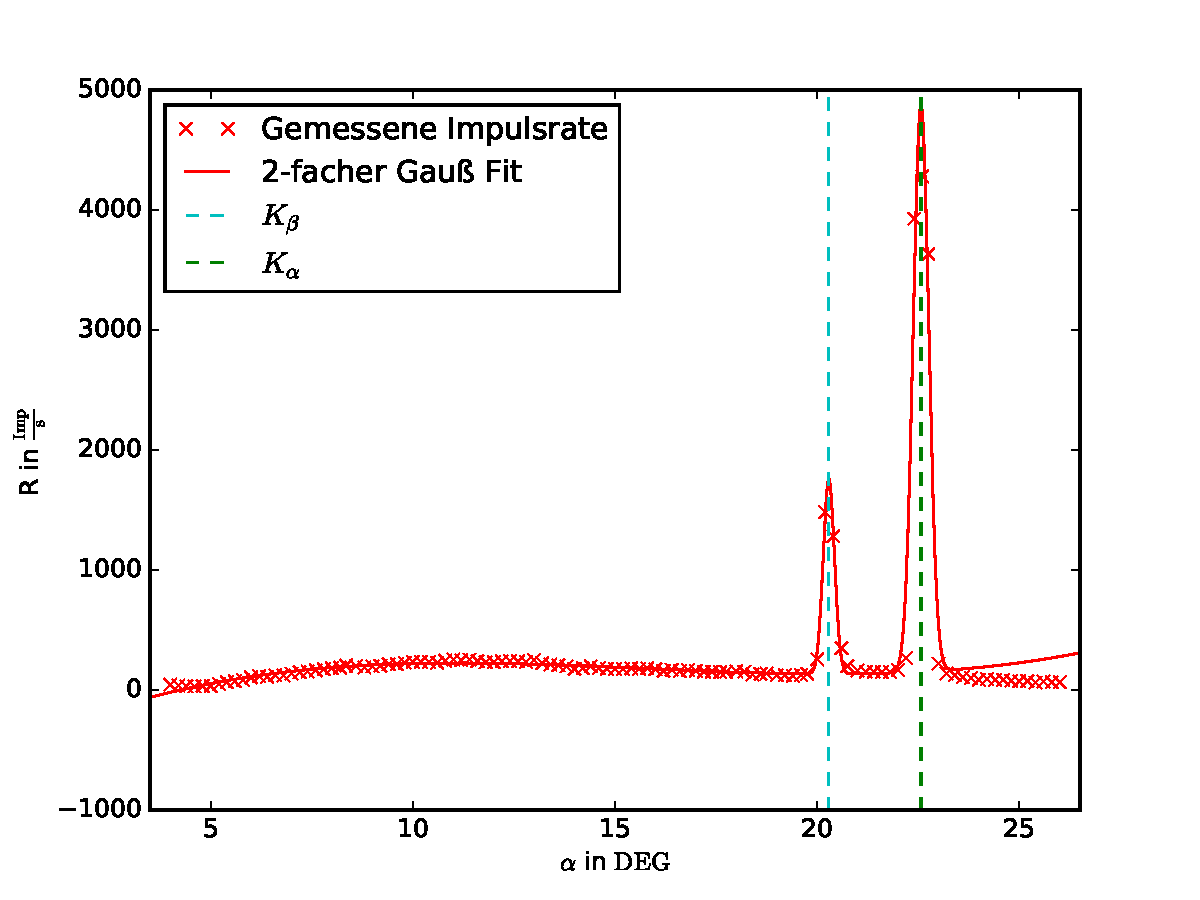
\includegraphics[width = 0.8\textwidth]{Python/MessungB.pdf}
  \caption{Gemessene Impulsrate einer Cu-Röntgenröhre.}
  \label{fig:MessungB}
\end{figure}

\begin{table}
  \centering
  \caption{Die für den Untergrund verwendeten Messdaten. }
  \label{tab:Untergrund}
  \begin{tabular}{c c | c c | c c}
    \toprule
    2$\vartheta$ in deg & N in $\frac{\su{Imp}}{\su{s}}$ & 2$\vartheta$ in deg &
    N in $\frac{\su{Imp}}{\su{s}}$ & 2$\vartheta$ in deg & N in $\frac{\su{Imp}}{\su{s}}$ \\
    \midrule
     8.0	& 45.0  & 21.2 & 227.0 & 34.4	& 153.0 \\
     8.4	& 38.0  & 21.6 & 245.0 & 34.8	& 153.0 \\
     8.8	& 31.0  & 22.0 & 254.0 & 35.2 & 147.0 \\
     9.2	& 31.0  & 22.4 & 247.0 & 35.5 & 153.0 \\
     9.6	& 33.0  & 22.8 & 253.0 & 36.0 & 155.0 \\
     10.0	& 34.0  & 23.2 & 240.0 & 36.4 & 152.0 \\
     10.4	& 50.0  & 23.6 & 232.0 & 36.8 & 130.0 \\
     10.8	& 64.0  & 24.0 & 233.0 & 37.2 & 134.0 \\
     11.2	& 73.0  & 24.4 & 239.0 & 37.5 & 137.0 \\
     11.6	& 85.0  & 24.8 & 241.0 & 38.0 & 123.0 \\
     12.0	& 105.0 & 25.2 & 239.0 & 38.4 & 124.0 \\
     12.4	& 114.0 & 25.6 & 234.0 & 38.8 & 119.0 \\
     12.8	& 110.0 & 26.0 & 250.0 & 39.2 & 126.0 \\
     13.2	& 123.0 & 26.4 & 224.0 & 39.5 & 136.0 \\
     13.6	& 121.0 & 26.8 & 213.0 & 42.4 & 152.0 \\
     14.0	& 136.0 & 27.2 & 207.0 & 42.8 & 153.0 \\
     14.4	& 149.0 & 27.6 & 197.0 & 43.2 & 147.0 \\
     14.8	& 154.0 & 28.0 & 176.0 & 43.6 & 150.0 \\
     15.2	& 163.0 & 28.4 & 181.0 & 44.0 & 167.0 \\
     15.6	& 172.0 & 28.8 & 197.0 & 46.8 & 124.0 \\
     16.0	& 181.0 & 29.2 & 182.0 & 47.2 & 108.0 \\
     16.4	& 187.0 & 29.6 & 177.0 & 47.6 & 100.0 \\
     16.7	& 204.0 & 30.0 & 176.0 & 48.0 & 86.0  \\
     17.2	& 200.0 & 30.4 & 174.0 & 48.4 & 92.0  \\
     17.6	& 188.0 & 30.8 & 180.0 & 48.8 & 86.0  \\
     18.0	& 197.0 & 31.2 & 176.0 & 49.2 & 86.0  \\
     18.4	& 202.0 & 31.6 & 181.0 & 49.6 & 77.0  \\
     18.8	& 215.0 & 32.0 & 173.0 & 50.0 & 72.0  \\
     19.2	& 216.0 & 32.4 & 159.0 & 50.4 & 75.0  \\
     19.6	& 227.0 & 32.8 & 169.0 & 50.8 & 61.0  \\
     20.0	& 236.0 & 33.2 & 158.0 & 51.2 & 71.0  \\
     20.4	& 235.0 & 33.6 & 167.0 & 51.6 & 64.0  \\
     20.8	& 235.0 & 34.0 & 160.0 & 52.0 & 65.0  \\
    \bottomrule
  \end{tabular}
\end{table}


\begin{table}
  \centering
  \caption{Die für den linke Gauß-Fit vorgesehenen Messdaten. }
  \label{tab:Gauß1}
  \begin{tabular}{c c | c c | c c}
    \toprule
    $\vartheta$ in deg & N in $\frac{\su{Imp}}{\su{s}}$ & $\vartheta$ in deg &
    N in $\frac{\su{Imp}}{\su{s}}$ & $\vartheta$ in deg & N in $\frac{\su{Imp}}{\su{s}}$ \\
    \midrule
    36.0 & 155.0 & 38.8 & 119.0  & 41.5 & 199.0 \\
    36.4 & 152.0 & 39.2 & 126.0  & 42.0 & 163.0 \\
    36.8 & 130.0 & 39.5 & 136.0  & 42.4 & 152.0 \\
    37.2 & 134.0 & 40.0 & 255.0  & 42.8 & 153.0 \\
    37.5 & 137.0 & 40.4 & 1483.0 & 43.2 & 147.0 \\
    38.0 & 123.0 & 40.8 & 1282.0 & 43.6 & 150.0 \\
    38.4 & 124.0 & 41.2 & 349.0  & 44.0 & 167.0 \\
    \bottomrule
  \end{tabular}
\end{table}


\newpage %%%%%%%%%%%%%%%%%%%%%%%%%%%%%%%%%%%%%%%%%%%%%%%%%%%%%%%%%%%%%%%%%%%%%%%

Zuletzt kann mithilfe der Daten in einem Winkelbereich von $\vartheta$ $\in$
[4 °, 7 °] (Tabelle \ref{tab:Messung3.2}) noch die maximale Energie des
Röntgenspektrums bestimmt werden. Dafür wird nur ein Teil der gemessenen
Winkel ($\vartheta$ $\in$ [$\ang{4.8}$, $\ang{6.2}$]) verwendet,
um einen linearen Fit gemäß Formel \eqref{eqn:FitEmax} durchzuführen. Der
gesuchte Winkel ist der Anfang des Bremsberges. Das Ende des Bremsberges
kann bei den gemessenen Daten nicht beobachtet werden. Die verwendeten Messdaten
und die berechnete Nullstelle sind noch einmal in Abbildung \ref{fig:Emax}
dargestellt.

\begin{equation}
  \vartheta(x) = A \cdot x + B
  \label{eqn:FitEmax}
\end{equation}

Für die Parameter ergeben sich dabei die folgenden Werte:

\begin{align*}
  A &= (59 \pm 5) \, \si{\frac{Imp}{s\cdot \alpha}} \\
  B &= (-255 \pm 27) \, \si{\frac{Imp}{s}}
\end{align*}

Aus den beiden Parametern kann dann der Winkel bestimmt werden, bei dem
die Impulsrate den Wert 0 annimmt. Mithilfe von Formeln \eqref{eqn:Lambda}
und \eqref{eqn:Energie} kann dann die maximale Energie des verwendeten
Röntgenspektrums bestimmt werden.

\begin{align*}
  \vartheta\ua{E\ua{max}} &= - \frac{B}{A} = (4.3 \pm 0.6) \, ° \\
  \lambda\ua{E\ua{max}} &= (3.1 \pm 0.4)  \cdot 10^{-11} \, \si{m} \\
  E\ua{max} &= (4.1 \pm 0.5) \cdot 10^{4}\, \si{eV}
\end{align*}

\begin{table}
  \centering
  \caption{Gemessene Impulsraten N bei Messung 3.2.}
  \label{tab:Messung3.2}
  \begin{tabular}{c c | c c}
    \toprule
    2$\vartheta$ in deg & N in $\frac{\su{Imp}}{\su{s}}$ &
    2$\vartheta$ in deg & N in $\frac{\su{Imp}}{\su{s}}$  \\
    \midrule
     8.0 & 45.0 & 11.2 & 73.0  \\
     8.4 & 38.0 & 11.6 & 85.0  \\
     8.8 & 31.0 & 12.0 & 105.0 \\
     9.2 & 31.0 & 12.4 & 114.0 \\
     9.6 & 33.0 & 12.8 & 110.0 \\
    10.0 & 34.0 & 13.2 & 123.0 \\
    10.4 & 50.0 & 13.6 & 121.0 \\
    10.8 & 64.0 & 14.0 & 136.0 \\
    \bottomrule
  \end{tabular}
\end{table}


\begin{figure}
  \centering
  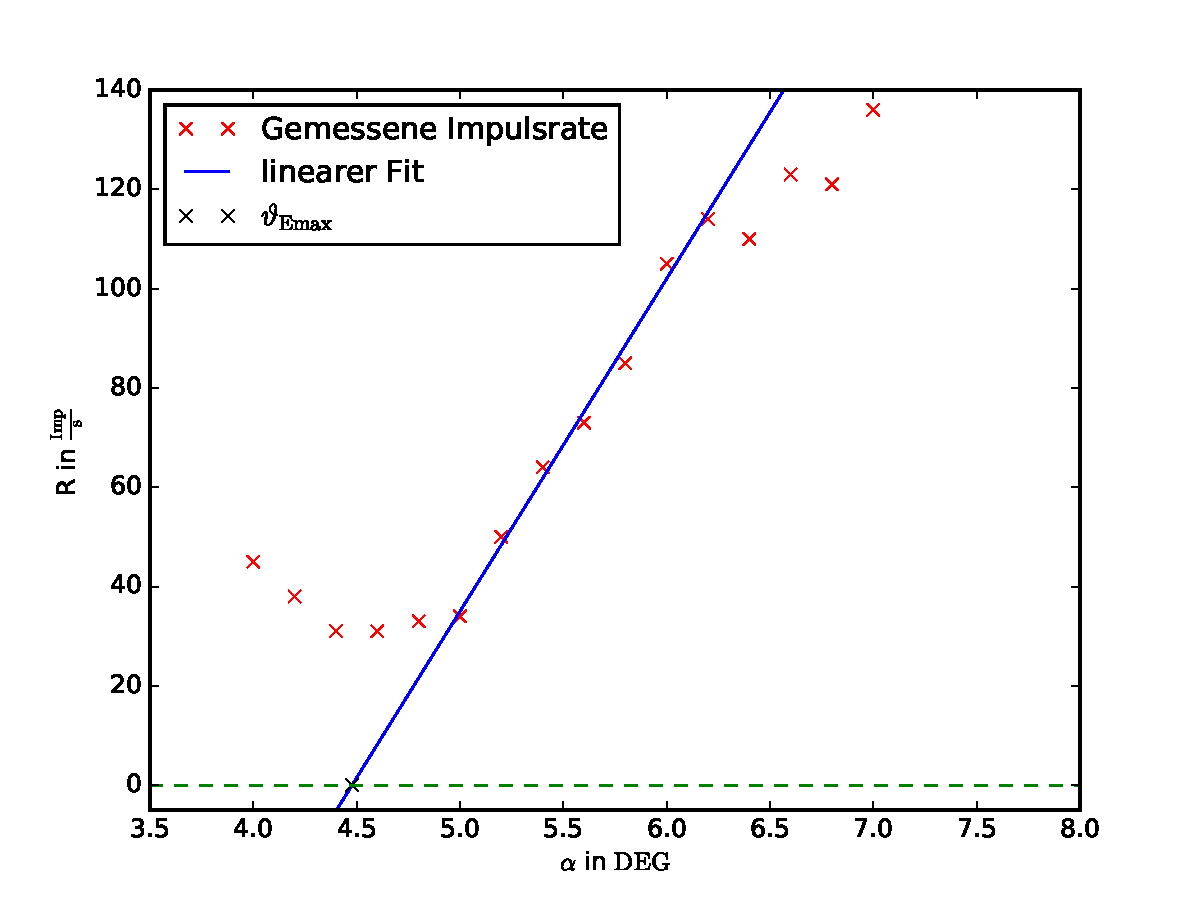
\includegraphics[width = 0.8\textwidth]{Python/SpektrumEnergie.pdf}
  \caption{Messdaten zu Bestimmung der maximalen Energie}
  \label{fig:Emax}
\end{figure}



\newpage %%%%%%%%%%%%%%%%%%%%%%%%%%%%%%%%%%%%%%%%%%%%%%%%%%%%%%%%%%%%%%%%%%%%%%%%%%%%%%%%%%%%%%%%55

\subsection{Das Absorptionsspektrum}

Für die Untersuchung des Absorptionsspektrums verschiedener Materialien werden in dem
2:1 Koppelmodus die folgenden Einstellungen verwendet:

\begin{align*}
  \increment\vartheta &= 0.1 \,° \\
  \increment t     &= \SI{20}{s} .
\end{align*}

Das Messintervall wird dabei für jedes Material unabhängig gewählt. Für die
Berechnung der Abschirmkonstante wird Formel \eqref{eqn:Bindungsenergie} umgestellt,
so dass sich die folgende Relation ergibt.  $\alpha$
beschreibt dabei die Sommerfeldsche Feinstrukturkonstante.

\begin{equation}
  \sigma\ua{K} = Z - \sqrt{ \frac{E\ua{max}}{R\ua{\infty}} - \frac{\alpha^4 Z^4}{4}}
  \label{eqn:Abschirmkonst}
\end{equation}

%\newpage %%%%%%%%%%%%%%%%%%%%%%%%%%%%%%%%%%%%%%%%%%%%%%%%%%%%%%%%%%%%%%%%%%%%%%%%%%%%%%%%%%%%%%%%55

\subsubsection{Germanium}

Für Germanium wird ein Messintervall von $\vartheta$ $\in$ [14 °, 18 °] verwendet.
Mithilfe der Daten aus Tabelle \ref{tab:Germanium} (grafisch siehe Abbildung
\ref{fig:Germanium})
kann für Germanium nun die Absorptionsenergie (Formel \eqref{eqn:Energie})
der K-Kante bestimmt werden sowie
die daraus resultierende Abschirmkonstante nach Formel \eqref{eqn:Abschirmkonst}.
Die für die Berechnung
der Werte verwendete Ordnungszahl ist 32.

\begin{align*}
  \vartheta\ua{GE} &= 16.15 \, ° \\
  \lambda\ua{GE,min} &= 1.12 \cdot 10^{-10} \, \si{m} \\
  E\ua{GE,max} &= 11066 \, \si{eV} \\
  \sigma\ua{GE} &= 3.72
\end{align*}

\begin{figure}
  \centering
  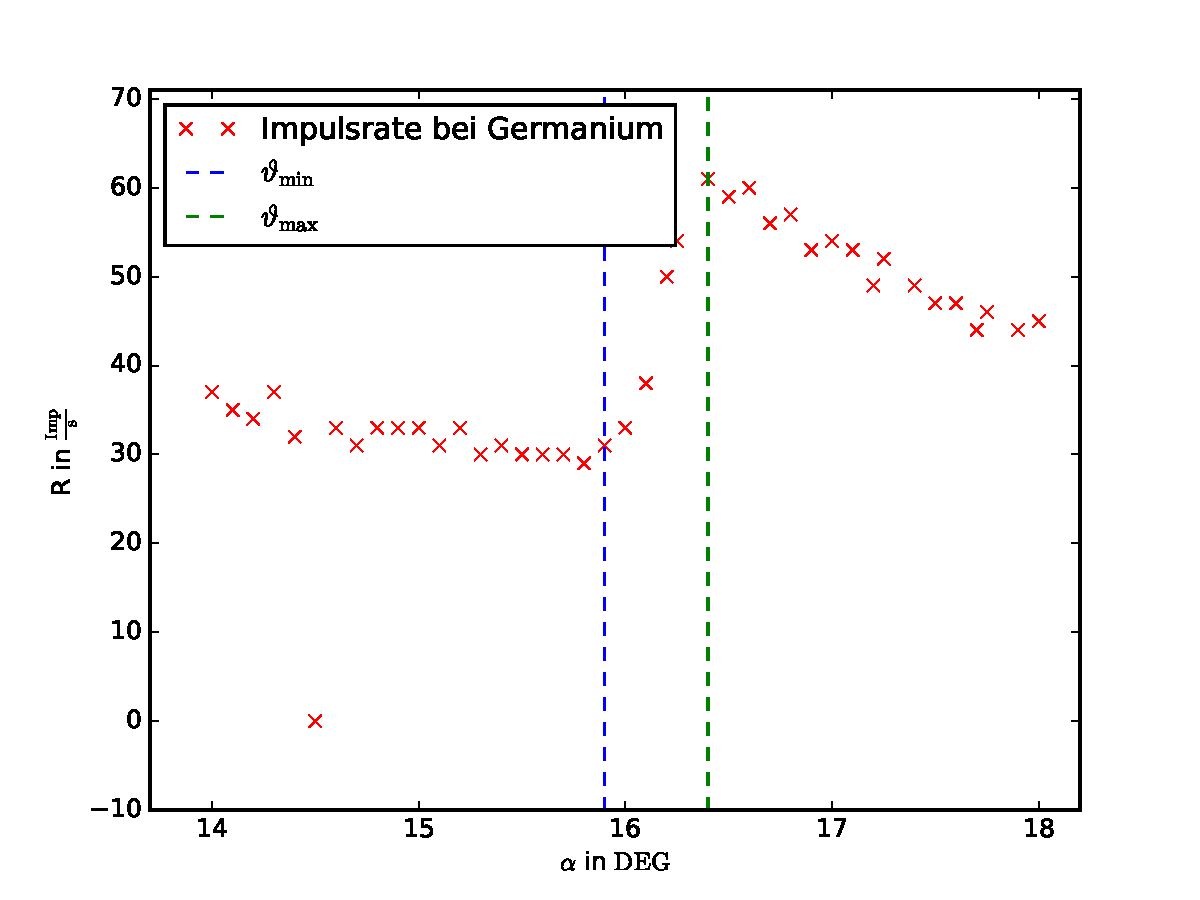
\includegraphics[width = 0.8\textwidth]{Python/Germanium.pdf}
  \caption{Gemessenes Absorptionsspektrum bei Germanium.}
  \label{fig:Germanium}
\end{figure}


\begin{table}
  \centering
  \caption{Gemessene Impulsrate N bei Germanium.}
  \label{tab:Germanium}
  \begin{tabular}{c c | c c | c c}
    \toprule
    $\vartheta$ in deg & N in $\frac{\su{Imp}}{\su{s}}$ & $\vartheta$ in deg &
    N in $\frac{\su{Imp}}{\su{s}}$ & $\vartheta$ in deg & N in $\frac{\su{Imp}}{\su{s}}$ \\
    \midrule
    28.0 & 37.0 & 30.8 & 31.0 & 33.6 & 57.0 \\
    28.2 & 35.0 & 31.0 & 30.0 & 33.8 & 53.0 \\
    28.4 & 34.0 & 31.2 & 30.0 & 34.0 & 54.0 \\
    28.6 & 37.0 & 31.4 & 30.0 & 34.2 & 53.0 \\
    28.8 & 32.0 & 31.6 & 29.0 & 34.4 & 49.0 \\
    29.0 & 0.0  & 31.8 & 31.0 & 34.5 & 52.0 \\
    29.2 & 33.0 & 32.0 & 33.0 & 34.8 & 49.0 \\
    29.4 & 31.0 & 32.2 & 38.0 & 35.0 & 47.0 \\
    29.6 & 33.0 & 32.4 & 50.0 & 35.2 & 47.0 \\
    29.8 & 33.0 & 32.5 & 54.0 & 35.4 & 44.0 \\
    30.0 & 33.0 & 32.8 & 61.0 & 35.5 & 46.0 \\
    30.2 & 31.0 & 33.0 & 59.0 & 35.8 & 44.0 \\
    30.4 & 33.0 & 33.2 & 60.0 & 36.0 & 45.0 \\
    30.6 & 30.0 & 33.4 & 56.0 &      &      \\
    \bottomrule
  \end{tabular}
\end{table}


Da die Berechnung der Werte für alle Materialien gleich erfolgt, werden im Folgenden
lediglich die Tabellen, Graphen sowie Ergebniss für Zink, Zirkonium, Strontium und
Brom vorgestellt.

\newpage %%%%%%%%%%%%%%%%%%%%%%%%%%%%%%%%%%%%%%%%%%%%%%%%%%%%%%%%%%%%%%%%%%%%%%%%%%

\subsubsection{Brom}

Für Brom wird ein Messintervall von $\vartheta$ $\in$ [11 °, 15 °] gewählt.
Die Ordnungszahl ist 35. Die gemessenen Werte sind in Tabelle \ref{tab:Brom}
sowie grafisch in Abbildung \ref{fig:Brom} dargestellt.

\begin{align*}
  \vartheta\ua{BR} &= 13.2 \,° \\
  \lambda\ua{BR,min} &= 9.20 \cdot 10^{-10} \, \si{m} \\
  E\ua{BR,max} &= 13480 \, \si{eV} \\
  \sigma\ua{BR} &= 3.84
\end{align*}

\begin{figure}
  \centering
  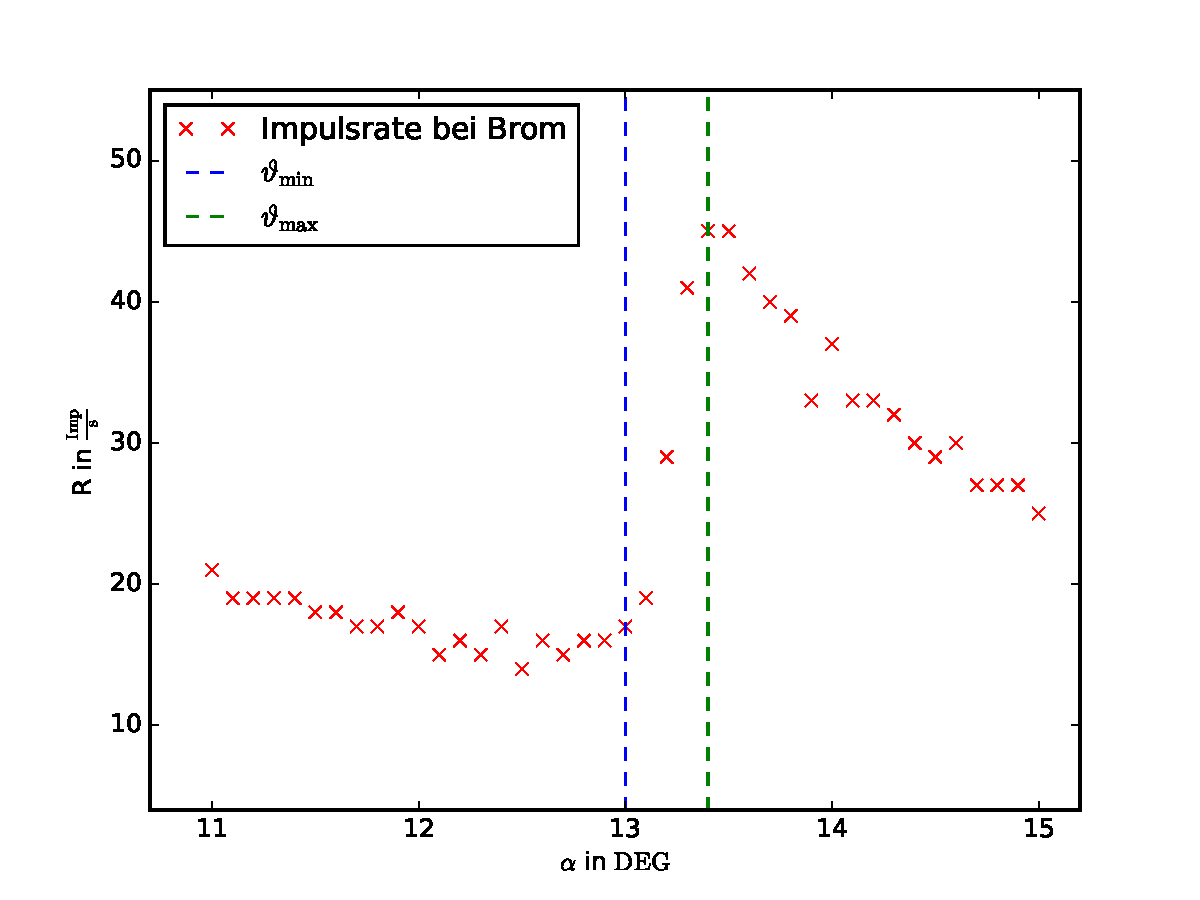
\includegraphics[width = 0.8\textwidth]{Python/Brom.pdf}
  \caption{Gemessenes Absorptionsspektrum bei Brom.}
  \label{fig:Brom}
\end{figure}

\begin{table}
  \centering
  \caption{Gemessene Impulsrate N bei Brom.}
  \label{tab:Brom}
  \begin{tabular}{c c | c c | c c}
    \toprule
    2$\vartheta$ in deg & N in $\frac{\su{Imp}}{\su{s}}$ & 2$\vartheta$ in deg &
    N in $\frac{\su{Imp}}{\su{s}}$ & 2$\vartheta$ in deg & N in $\frac{\su{Imp}}{\su{s}}$ \\
    \midrule
    22.0 & 21.0 & 24.8 & 17.0 & 27.6 & 39.0 \\
    22.2 & 19.0 & 25.0 & 14.0 & 27.8 & 33.0 \\
    22.4 & 19.0 & 25.2 & 16.0 & 28.0 & 37.0 \\
    22.6 & 19.0 & 25.4 & 15.0 & 28.2 & 33.0 \\
    22.8 & 19.0 & 25.6 & 16.0 & 28.4 & 33.0 \\
    23.0 & 18.0 & 25.8 & 16.0 & 28.6 & 32.0 \\
    23.2 & 18.0 & 26.0 & 17.0 & 28.8 & 30.0 \\
    23.4 & 17.0 & 26.2 & 19.0 & 29.0 & 29.0 \\
    23.6 & 17.0 & 26.4 & 29.0 & 29.2 & 30.0 \\
    23.8 & 18.0 & 26.6 & 41.0 & 29.4 & 27.0 \\
    24.0 & 17.0 & 26.8 & 45.0 & 29.6 & 27.0 \\
    24.2 & 15.0 & 27.0 & 45.0 & 29.8 & 27.0 \\
    24.4 & 16.0 & 27.2 & 42.0 & 30.0 & 25.0 \\
    24.6 & 15.0 & 27.4 & 40.0 &      &      \\
    \bottomrule
  \end{tabular}
\end{table}


\newpage %%%%%%%%%%%%%%%%%%%%%%%%%%%%%%%%%%%%%%%%%%%%%%%%%%%%%%%%%%%%%%%%%%%%%%%%%%

\subsubsection{Zirkonium}

Das gewählte Messintervall von Zirkonium ist $\vartheta$ $\in$ [8 °, 12 °]. Die
Ordnungszahl von Zirkonium ist 40. Alle Daten sind in Tabelle \ref{tab:Zirkonium}
sowie Abbildung \ref{fig:Zirkonium} dargestellt.

\begin{align*}
  \vartheta\ua{ZR} &= 9.85 \,° \\
  \lambda\ua{ZR,min} &= 6.89 \cdot 10^{-11} \, \si{m} \\
  E\ua{ZR,max} &= 17993 \, \si{eV} \\
  \sigma\ua{ZR} &= 4.10
\end{align*}

\begin{figure}
  \centering
  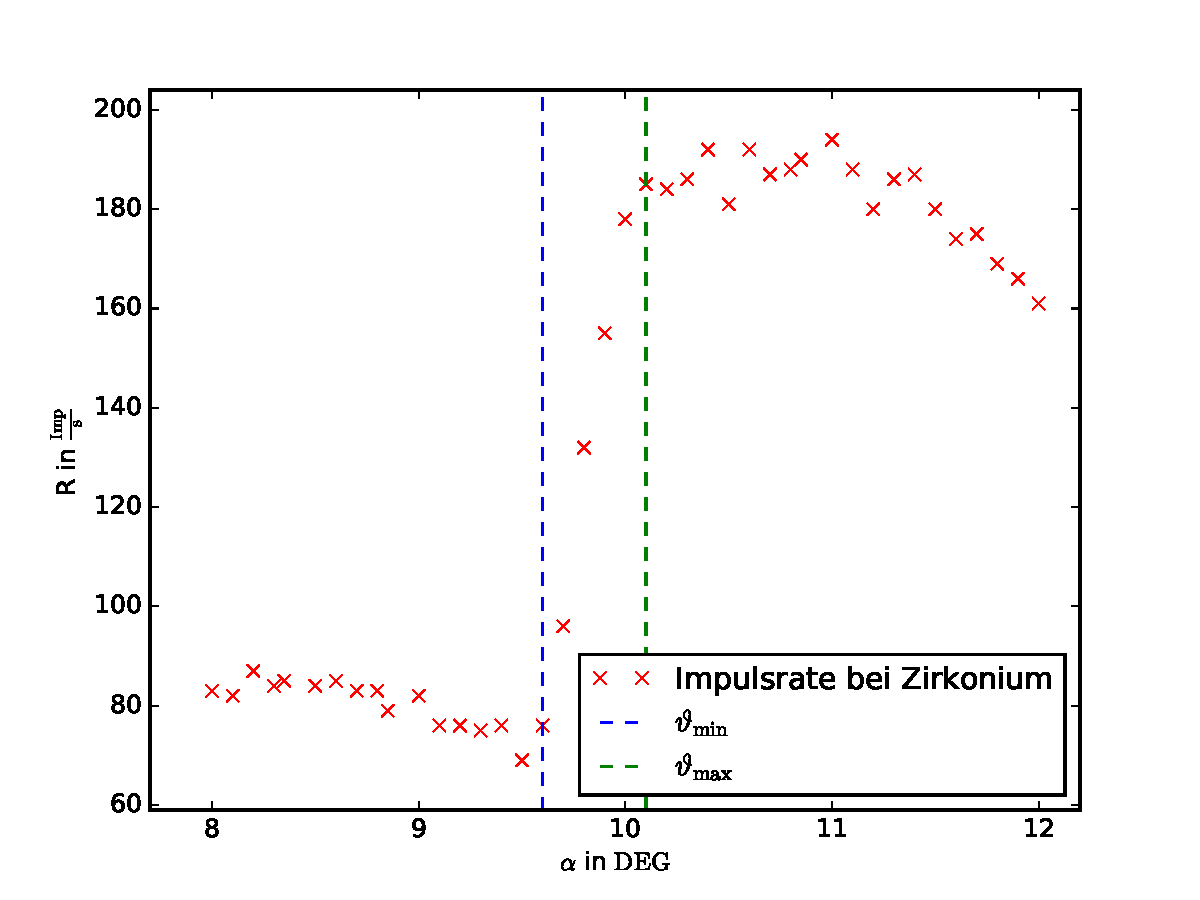
\includegraphics[width = 0.8\textwidth]{Python/Zirkonium.pdf}
  \caption{Gemessenes Absorptionsspektrum bei Zirkonium.}
  \label{fig:Zirkonium}
\end{figure}

\begin{table}
  \centering
  \caption{Gemessene Impulsrate N bei Zirkonium.}
  \label{tab:Zirkonium}
  \begin{tabular}{c c | c c | c c}
    \toprule
    2$\vartheta$ in deg & N in $\frac{\su{Imp}}{\su{s}}$ & 2$\vartheta$ in deg &
    N in $\frac{\su{Imp}}{\su{s}}$ & 2$\vartheta$ in deg & N in $\frac{\su{Imp}}{\su{s}}$ \\
    \midrule
    16.0 & 83.0 & 18.8 & 76.0  & 21.6 & 188.0 \\
    16.2 & 82.0 & 19.0 & 69.0  & 21.7 & 190.0 \\
    16.4 & 87.0 & 19.2 & 76.0  & 22.0 & 194.0 \\
    16.6 & 84.0 & 19.4 & 96.0  & 22.2 & 188.0 \\
    16.7 & 85.0 & 19.6 & 132.0 & 22.4 & 180.0 \\
    17.0 & 84.0 & 19.8 & 155.0 & 22.6 & 186.0 \\
    17.2 & 85.0 & 20.0 & 178.0 & 22.8 & 187.0 \\
    17.4 & 83.0 & 20.2 & 185.0 & 23.0 & 180.0 \\
    17.6 & 83.0 & 20.4 & 184.0 & 23.2 & 174.0 \\
    17.7 & 79.0 & 20.6 & 186.0 & 23.4 & 175.0 \\
    18.0 & 82.0 & 20.8 & 192.0 & 23.6 & 169.0 \\
    18.2 & 76.0 & 21.0 & 181.0 & 23.8 & 166.0 \\
    18.4 & 76.0 & 21.2 & 192.0 & 24.0 & 161.0 \\
    18.6 & 75.0 & 21.4 & 187.0 &      &       \\
    \bottomrule
  \end{tabular}
\end{table}


\newpage %%%%%%%%%%%%%%%%%%%%%%%%%%%%%%%%%%%%%%%%%%%%%%%%%%%%%%%%%%%%%%%%%%%%%%%%%%

\subsubsection{Strontium}

Strontium besitzt die Ordnungszahl 38. Für die Messung wird ein Intervalle von
$\vartheta$ $\in$ [9 °, 13 °] betrachtet. Die Ergebnisse sind in Tabelle \ref{tab:Strontium}
und Abbildung \ref{fig:Strontium} dargestellt.

\begin{align*}
  \vartheta\ua{SR} &= 11.0 \,° \\
  \lambda\ua{SR,min} &= 7.69 \cdot 10^{-11} \, \si{m} \\
  E\ua{SR,max} &= 16132 \, \si{eV} \\
  \sigma\ua{SR} &= 3.96
\end{align*}

\begin{figure}
  \centering
  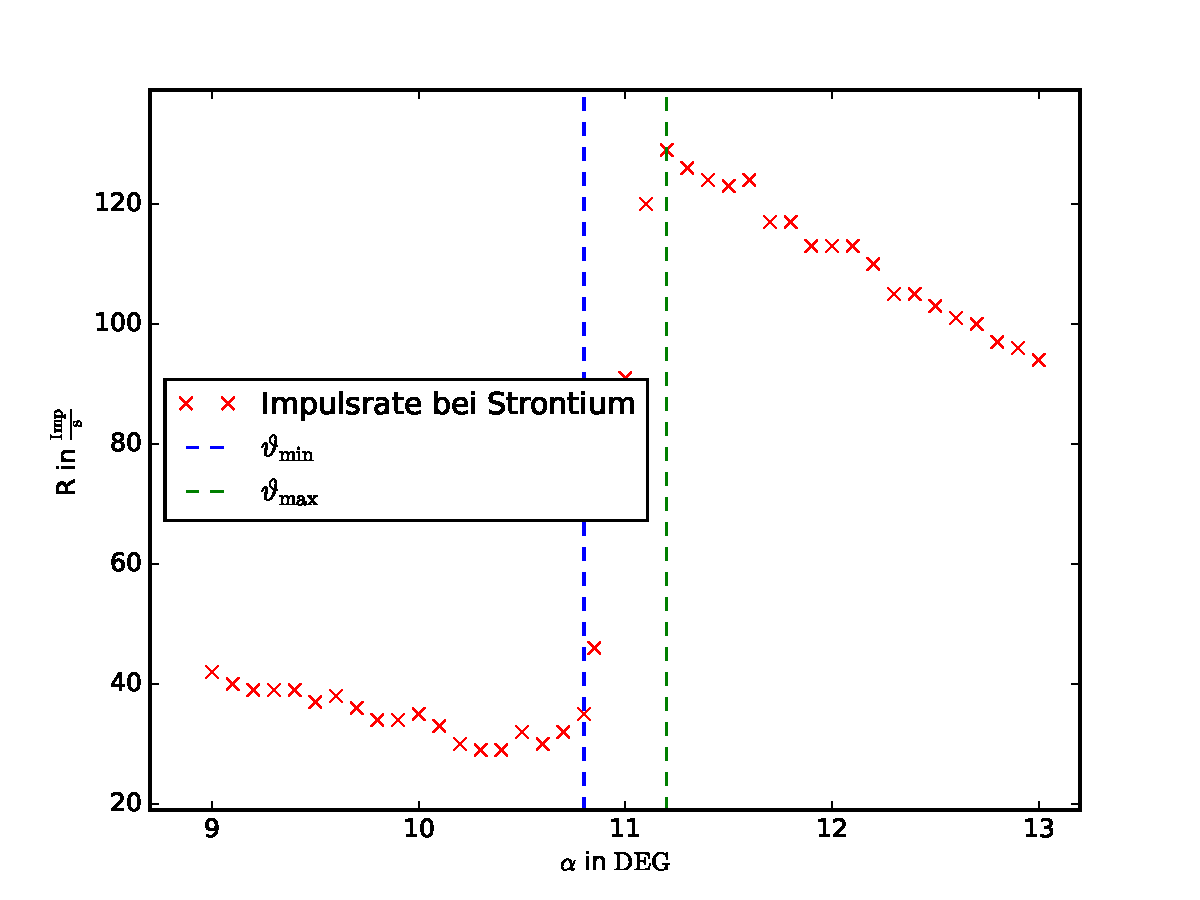
\includegraphics[width = 0.8\textwidth]{Python/Strontium.pdf}
  \caption{Gemessenes Absorptionsspektrum bei Strontium.}
  \label{fig:Strontium}
\end{figure}

\begin{table}
  \centering
  \caption{Gemessene Impulsrate N bei Strontium.}
  \label{tab:Strontium}
  \begin{tabular}{c c | c c | c c}
    \toprule
    2$\vartheta$ in deg & N in $\frac{\su{Imp}}{\su{s}}$ & 2$\vartheta$ in deg &
    N in $\frac{\su{Imp}}{\su{s}}$ & 2$\vartheta$ in deg & N in $\frac{\su{Imp}}{\su{s}}$ \\
    \midrule
    18.0 & 42.0 & 20.8 & 29.0  & 23.6 & 117.0 \\
    18.2 & 40.0 & 21.0 & 32.0  & 23.8 & 113.0 \\
    18.4 & 39.0 & 21.2 & 30.0  & 24.0 & 113.0 \\
    18.6 & 39.0 & 21.4 & 32.0  & 24.2 & 113.0 \\
    18.8 & 39.0 & 21.6 & 35.0  & 24.4 & 110.0 \\
    19.0 & 37.0 & 21.7 & 46.0  & 24.6 & 105.0 \\
    19.2 & 38.0 & 22.0 & 91.0  & 24.8 & 105.0 \\
    19.4 & 36.0 & 22.2 & 120.0 & 25.0 & 103.0 \\
    19.6 & 34.0 & 22.4 & 129.0 & 25.2 & 101.0 \\
    19.8 & 34.0 & 22.6 & 126.0 & 25.4 & 100.0 \\
    20.0 & 35.0 & 22.8 & 124.0 & 25.6 & 97.0  \\
    20.2 & 33.0 & 23.0 & 123.0 & 25.8 & 96.0  \\
    20.4 & 30.0 & 23.2 & 124.0 & 26.0 & 94.0  \\
    20.6 & 29.0 & 23.4 & 117.0 &      &       \\
    \bottomrule
  \end{tabular}
\end{table}


\newpage %%%%%%%%%%%%%%%%%%%%%%%%%%%%%%%%%%%%%%%%%%%%%%%%%%%%%%%%%%%%%%%%%%%%%%%%%%

\subsubsection{Zink}

Für Zink wird ein Messintervall von $\vartheta$ $\in$ [17 °, 21 °] gewählt. Die
Ordnungszahl von Zink ist 30. Alle verwerteten Daten sind in Tabelle \ref{tab:Zink}
sowie grafisch in Abbildung \ref{fig:Zink} dargestellt.

\begin{align*}
  \vartheta\ua{SR} &= 18.58 \,° \\
  \lambda\ua{SR,min} &= 1.28 \cdot 10^{-10} \, \si{m} \\
  E\ua{SR,max} &= 9663 \, \si{eV} \\
  \sigma\ua{SR} &= 3.55
\end{align*}

\begin{figure}
  \centering
  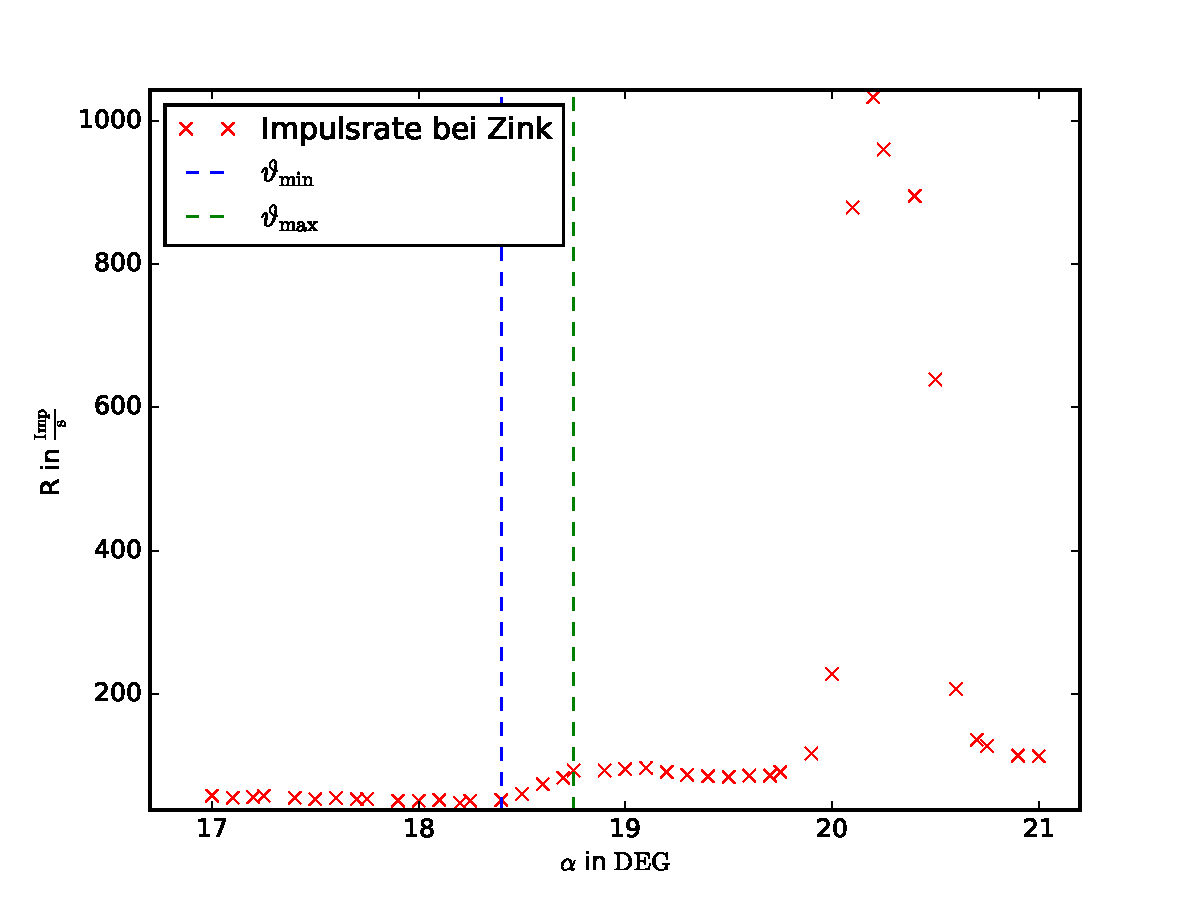
\includegraphics[width = 0.8\textwidth]{Python/Zink.pdf}
  \caption{Gemessenes Absorptionsspektrum bei Zink.}
  \label{fig:Zink}
\end{figure}

\begin{table}
  \centering
  \caption{Gemessene Impulsrate N bei Zink.}
  \label{tab:Zink}
  \begin{tabular}{c c | c c | c c}
    \toprule
    $\vartheta$ in deg & N in $\frac{\su{Imp}}{\su{s}}$ & $\vartheta$ in deg &
    N in $\frac{\su{Imp}}{\su{s}}$ & $\vartheta$ in deg & N in $\frac{\su{Imp}}{\su{s}}$ \\
    \midrule
    34.0 & 58.0 & 36.8 & 52.0 & 39.5 & 91.0   \\
    34.2 & 55.0 & 37.0 & 60.0 & 39.8 & 117.0  \\
    34.4 & 56.0 & 37.2 & 74.0 & 40.0 & 228.0  \\
    34.5 & 58.0 & 37.4 & 83.0 & 40.2 & 879.0  \\
    34.8 & 55.0 & 37.5 & 93.0 & 40.4 & 1033.0 \\
    35.0 & 53.0 & 37.8 & 93.0 & 40.5 & 960.0  \\
    35.2 & 55.0 & 38.0 & 95.0 & 40.8 & 895.0  \\
    35.4 & 53.0 & 38.2 & 97.0 & 41.0 & 639.0  \\
    35.5 & 53.0 & 38.4 & 91.0 & 41.2 & 207.0  \\
    35.8 & 51.0 & 38.6 & 87.0 & 41.4 & 136.0  \\
    36.0 & 51.0 & 38.8 & 85.0 & 41.5 & 127.0  \\
    36.2 & 52.0 & 39.0 & 84.0 & 41.8 & 114.0  \\
    36.4 & 48.0 & 39.2 & 86.0 & 42.0 & 113.0  \\
    36.5 & 51.0 & 39.4 & 86.0 &      &        \\
    \bottomrule
  \end{tabular}
\end{table}


\newpage %%%%%%%%%%%%%%%%%%%%%%%%%%%%%%%%%%%%%%%%%%%%%%%%%%%%%%%%%%%%%%%%%%%%%%%%%%

\subsubsection{Rydbergenergie}

Mithilfe der bestimmten Bindungsenergie kann nun gemäß Formel \eqref{eqn:Bindungsenergie}
die Rydbergenergie bestimmt werden. Dafür wird die Energie $\sqrt{E\ua{n}}$ gegen
die Ordnungszahl Z ausgetragen und gemäß der nachfolgenden Formeln (\eqref{eqn:RydbergFit1}
und \eqref{eqn:RydbergFit1}) eine lineare
Regression durchgeführt. Dabei wird aufgrund der Betrachtung der K-Kante $n$ = 1
gewählt.

\begin{align}
  \label{eqn:RydbergFit1}
  \sqrt{E\ua{n}} &=  \sqrt{R\ua{\infty}} \cdot Z  \\
  \label{eqn:RydbergFit2}
  f(x) &= A \dot c + B
\end{align}

\begin{figure}
  \centering
  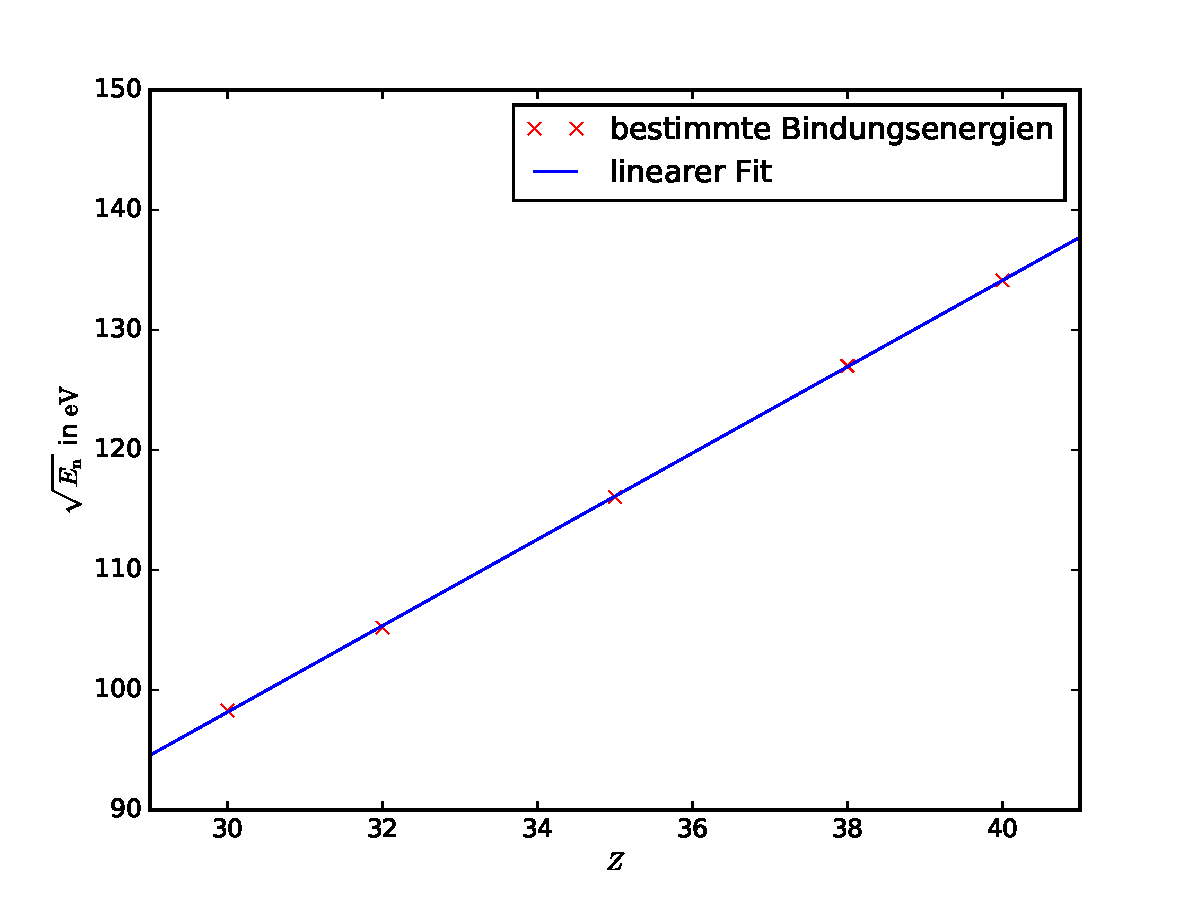
\includegraphics[width = 0.8\textwidth]{Python/Rydberg.pdf}
  \caption{Abhängigkeit der Bindungsenergie von der Ordnungszahl}
  \label{fig:Rydberg}
\end{figure}

Die lineare Regression ist noch einmal grafisch in Abbildung \ref{fig:Rydberg}
dargestellt. Dabei ergeben sich für die Parameter der linearen Regression
folgende Werte:

\begin{align*}
  A &= (3.60 \pm 0.2) \, \si{\sqrt{eV}} \\
  B &= (-9.8 \pm 0.6) \, \si{eV} \\
  Ryd\ua{exp} &= A^2 = (12.94 \pm 0.11) \si{eV}
\end{align*}

\newpage %%%%%%%%%%%%%%%%%%%%%%%%%%%%%%%%%%%%%%%%%%%%%%%%%%%%%%%%%%%%%%%%%%%%%%%%%%%%%%%%%%%%%%%%55

\subsubsection{Betrachtung der L-Kanten von Gold}

In dem letzten Teil des Experimentes werden noch einmal die $L\ua{II}$ und
$L\ua{III}$ betrachtet. Zur Messung wird ein Intervall von $\vartheta \, \in$
 [11 °, 17 °] gewählt. In $\increment \vartheta$ = 0.1 ° Schritten sowie mit einer
Integrationszeit von $\increment t$ = 20 $\su{s}$ wird das Intervall abgelaufen.
Die verwendeten Daten sind in
Tabelle \ref{tab:Gold} sowie grafisch in Abbildung \ref{fig:Gold} dargestellt.

\begin{table}
  \centering
  \caption{Gemessene Impulsrate N bei Gold.}
  \label{tab:Gold}
  \begin{tabular}{c c | c c | c c}
    \toprule
    2$\vartheta$ in deg & N in $\frac{\su{Imp}}{\su{s}}$ & 2$\vartheta$ in deg &
    N in $\frac{\su{Imp}}{\su{s}}$ & 2$\vartheta$ in deg & N in $\frac{\su{Imp}}{\su{s}}$ \\
    \midrule
    22.0 & 109.0 & 26.2 & 108.0 & 30.4 & 107.0 \\
    22.2 & 107.0 & 26.4 & 101.0 & 30.6 & 108.0 \\
    22.4 & 103.0 & 26.6 & 99.0  & 30.8 & 106.0 \\
    22.6 & 101.0 & 26.8 & 97.0  & 31.0 & 110.0 \\
    22.8 & 105.0 & 27.0 & 89.0  & 31.2 & 103.0 \\
    23.0 & 96.0  & 27.2 & 86.0  & 31.4 & 102.0 \\
    23.2 & 95.0  & 27.4 & 89.0  & 31.6 & 101.0 \\
    23.4 & 91.0  & 27.6 & 79.0  & 31.8 & 105.0 \\
    23.6 & 94.0  & 27.8 & 81.0  & 32.0 & 97.0  \\
    23.8 & 90.0  & 28.0 & 76.0  & 32.2 & 95.0  \\
    24.0 & 88.0  & 28.2 & 78.0  & 32.4 & 95.0  \\
    24.2 & 89.0  & 28.4 & 75.0  & 32.5 & 90.0  \\
    24.4 & 86.0  & 28.6 & 73.0  & 32.8 & 90.0  \\
    24.6 & 89.0  & 28.8 & 74.0  & 33.0 & 87.0  \\
    24.8 & 91.0  & 29.0 & 73.0  & 33.2 & 86.0  \\
    25.0 & 90.0  & 29.2 & 76.0  & 33.4 & 86.0  \\
    25.2 & 93.0  & 29.4 & 71.0  & 33.6 & 87.0  \\
    25.4 & 92.0  & 29.6 & 73.0  & 33.8 & 84.0  \\
    25.6 & 90.0  & 29.8 & 82.0  & 34.0 & 82.0  \\
    25.8 & 99.0  & 30.0 & 92.0  &      &       \\
    26.0 & 107.0 & 30.2 & 101.0 &      &       \\
    \bottomrule
  \end{tabular}
\end{table}


\begin{figure}
  \centering
  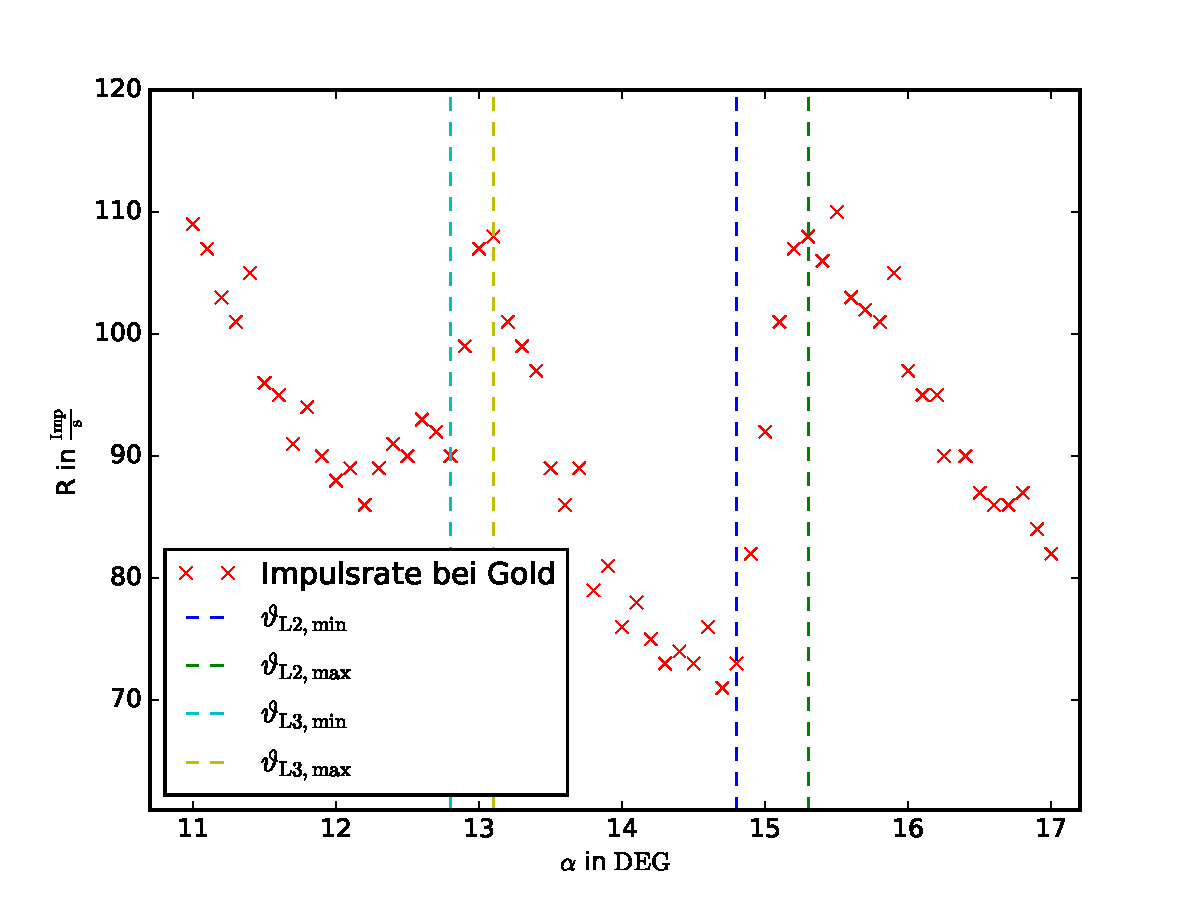
\includegraphics[width = 0.8\textwidth]{Python/Gold.pdf}
  \caption{Gemessene Impulsrate bei Gold.}
  \label{fig:Gold}
\end{figure}

Für die beiden Kanten ergeben sich damit folgende Werte:

\begin{align*}
  \vartheta\ua{AU,L\ua{II}} &= 12.95 ° \\
  \lambda\ua{AU,L\ua{II}} &= 9.027 \cdot 10^{-11} \, \si{m} \\
  E\ua{AU,L\ua{II}} &= 13735 \, \si{eV}
\end{align*}

\begin{align*}
  \vartheta\ua{AU,L\ua{III}} &= 15.05 ° \\
  \lambda\ua{AU,L\ua{III}} &= 1.046 \cdot 10^{-10} \, \si{m} \\
  E\ua{AU,L\ua{III}} &= 11854 \, \si{eV}
\end{align*}

Aus den beiden Energiewerten bzw. der Energiedifferent lässt sich nun
gemäß Formel \eqref{eqn:sigma_L} die Abschirmkonstante der $L$-Kante bestimmen.

\begin{equation}
  \sigma\ua{L} = (2.13 \pm 0.15)
\end{equation}

Der angegebene Fehler entspringt dabei der hier verwendeten experimentell bestimmten
Rydbergenergie (3.3.6) und wird durch die Gaußsche Fehlerfortpflanzung weitergegeben:

\begin{equation}
  \increment \sigma\ua{L} = \increment\ua{Ryd\ua{exp}} \cdot \frac{\partial \sigma\ua{L}}{\partial \su{Ryd\ua{exp}}} .
\end{equation}

\newpage %%%%%%%%%%%%%%%%%%%%%%%%%%%%%%%%%%%%%%%%%%%%%%%%%%%%%%%%%%%%%%%%%%%%%%%%%%

\section{Diskussion}

In Tabelle \ref{tab:DiskussionEnergie} sind noch einmal alle bestimmten Energiewerte
der verschiedenen Stoffe im Vergleich zum Literaturwert dargestellt. Dabei zeigt sich,
dass die Abweichungen alle in einem relativ kleinen Bereich von maximal ca. 7 $\%$
liegen.

\begin{table}
  \centering
  \caption{Vergleich der bestimmten Energie-Werte mit den Litarturwerten.\cite{anleitung02}}
  \label{tab:DiskussionEnergie}
  \begin{tabular}{c c c c c }
    \toprule
    Material & Linie & $E\ua{n,lit}$ in $\si{keV}$ & $E\ua{n,exp}$ in $\si{keV}$
    & $\increment E\ua{n}$ in $\%$ \\
    \midrule
    Kupfer     & $K\ua{\alpha}$ &  8.06 &  8.02 & 4.96  \\
    Kupfer     & $K\ua{\beta}$  &  8.92 &  8.88 & 4.48  \\
    Zink       & $K$            &  9.65 &  9.66 & 1.04  \\
    Germanium  & $K$            & 11.10 & 11.07 & 2.73  \\
    Brom       & $K$            & 13.47 & 13.48 & 7.42  \\
    Strontium  & $K$            & 16.10 & 16.13 & 1.86  \\
    Zirkonium  & $K$            & 17.99 & 17.99 & 0  \\
    Gold       & $L\ua{II}$     & 13.75 & 13.75 & 0  \\
    Gold       & $L\ua{III}$    & 11.93 & 11.85 & 6.71  \\
  \end{tabular}
\end{table}


In Abschnitt 3.2 wird das Auflösungsvermögen angesprochen. Die beiden K-Linien
hier können aufgrund der Energiedifferent ihrer Lagen noch differenziert dargestellt
werden. Im Vergleich mit der Theorie wird jedoch erkenntlich, dass das Auflösungsvermögen
nicht mehr ausreicht, um die $L\ua{I}$ und $L\ua{II}$ getrennt darzustellen.

In Abschnitt 3.2 wurde der Untergrund zudem nur durch ein Polynom 3.Grades genähert.
Weitaus genauer wäre eine Berechnung mittels der Shirley- oder Tougaard-Näherung
gewesen. Jedoch wurde aufgrund des hohen Aufwands auf die Anwendung dieser Methoden
verzichtet. Eine weiter Verbesserungsmöglichkeit für die Genauigkeit des Experimentes
wäre das Aufnehmen von mehr Messwerten im Bereich um das Impulsmaximum gewesen.

Der bei dem Versuch auftretenden Bremsberg wurde verwendet, um die maximale
Energie des verwendeten Röntgenspektrums zu bestimmen. Da nur durch wenige
Werte gefittet wurde, ist der Fehler im Vergleich zu den anderen bestimmten
Werten relativ groß.

Der theoretische Wert für die maximale Energie wäre aufgrund der gewählten
Beschleunigungsspannung $E\ua{max,lit}$ = $\SI{3.5e4}{eV}$. Dieser Wert liegt nicht
in dem Fehlerintervall des experimentell bestimmten $E\ua{max}$. Die Abweichung
ist einerseits statistischer bzw. systematischer Fehlernatur. Andererseits spielt
jedoch auch die Fermi-Dirac-Verteilung eine kleine Rolle, da manche Elektronen
nach dieser schon eine gewisse Anfangsenergie besitzen und anschließend noch
beschleunigt werden.

Der Bremsberg beginnt wie beschrieben bei $\vartheta\ua{E\ua{max}}$, jedoch ist
das Ende des Bremsberges auf dem Graphen \ref{fig:MessungB} nicht mehr erkenntlich.
Theoretisch wäre dies jedoch der Winkel, für den die Energie den Wert $\SI{0}{eV}$
annimmt.

Dier verschiedenen errechneten Abschirmkonstanten in Kapitel 3.3 können nun noch
mit den vorher berechneten Werten verglichen werden Tabelle \ref{tab:Abschirmkonstanten}.
Da diese Werte jedoch mit
Formel \eqref{eqn:Bindungsenergie_vereinfacht} bestimmt wurden, sind die experimentell
bestimmten Werte als genauer anzusehen, da hier die Formel \eqref{eqn:Bindungsenergie}
mit einer höheren Ordnung angewandt wurde. Bis auf die Werte von Zink zeigen sich
starke Abweichungen, jedoch sind die bereits oben verglichenen Energien nahezu identisch,
sodass diese Abweichungen auf die Rechenmethode zurückgeführt werden können.

\begin{table}
  \centering
  \caption{Vergleich der bestimmten Abschirmkonstanten mit den Litarturwerten. \cite{anleitung02}}
  \label{tab:Abschirmkonstanten}
  \begin{tabular}{c c c c  }
    \toprule
    Material & Linie & $\sigma\ua{lit}$ & $\sigma\ua{exp}$  \\
    \midrule
    Zink      & K & 3.56 & 3.55 \\
    Germanium & K & 3.42 & 3.72 \\
    Brom      & K & 3.52 & 3.84 \\
    Strontium & K & 3.59 & 3.96 \\
    Zirkonium & K & 3.63 & 4.10 \\
    \bottomrule
  \end{tabular}
\end{table}


Die in Abschnit 3.3.6 bestimmte Rydbergenergie weißt eine Abweichung von lediglich
ca. 5 $\%$ zum Literaturwert auf. Somit scheint auch hier die Messung ziemlich
genaue Messergebnisse zu liefern.

Da in Abschnitt 3.1 bei der Untersuchung der Bragg-Bedingung schon eine Abweichung
von 0.6 ° erkenntlich war, lassen sich der großteil der Abweichungen vermutlich
auf diese Ungenauigkeit (bzw. systematischen Fehler) zurückführen. Um bessere
Ergebnisse zu erzielen, müsste
hier vermutlich die Feinjustierung verbessert werden.

Abschließend lässt sich jedoch sagen, dass die verwendete Messapparatur alle
signifikanten Charakteristika des untersuchten Themas aufzeigt und relativ
kleine Fehler liefert.
